\chapter{Heavy Flavor Jet Tagging}
Jets that origin from the heavy flavor quarks c and b have characteristic properties compared to jets that origin from gluons or light flavor quarks, which are u, d, and s quarks. The properties are essentially determined through the bound state hadrons formed by the quarks and are explained in section \ref{sec:ch_tag_properties}. These properties can be used to distinguish the jets in respect of present quark flavors (tagging). This is done using a fully connected feed-forward MLP in the DeepCSV algorithm, which is explained in section \ref{sec:ch_deepCSV}. A more advanced DNN is used by the DeepFlavour algorithm that is described in \ref{sec:ch_deepFlavour}.

\section{Heavy Flavor Jet Properties}\label{sec:ch_tag_properties}
\begin{figure}
\centering
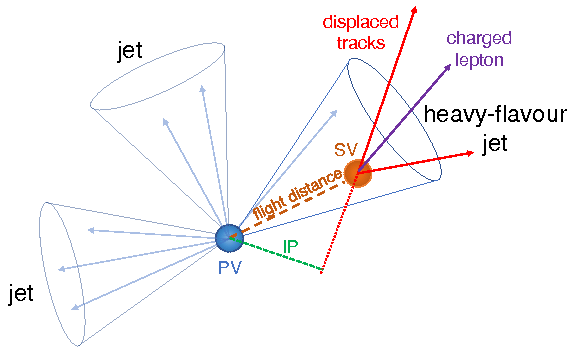
\includegraphics[width=0.6\textwidth]{chapter_5_tagging/SV.png}
\caption[Heavy Flavor Jet]{\textbf{A heavy flavor jet.} Several jet properties can be used to identify a heavy flavor jet. The main identifying properties are secondary vertices (SV) and displaced tracks with an impact parameter (IP) towards the primary vertex (PV).  Source: \cite{HeavyFlavorIdentification}}
\label{fig:ch_5_SV}
\end{figure}

B (C) hadrons have a lifetime in the order of 1.5\,ps (1\,ps) \cite{HeavyFlavorIdentification}, depending on their momentum, this results in a flight distance of some mm up to cm in the CMS detector. After this distance they decay at a secondary vertex (SV) where daughter particles arise. The SVs itself have characteristic properties, for example the vertex mass, which is the invariant mass of the SV. Another important variable is the flight distance (FD), defined as the distance from the PV to the SV. The FD can be measured in three spatial dimensions (3D), in the plane transverse to the beam line (2D) or in one dimension along the beam line (longitudinal). The tracks of the daughter particles can be propagated towards the beam line. The distance of their closest approach to the primary vertex is called impact parameter (IP). The daughter particles tend to have larger IPs compared to tacks that origin from the PV, they have displaced tracks. These aspects are outlined in figure \ref{fig:ch_5_SV}. The IP can be measured similar to the FD in 3D, 2D or in longitudinal direction. The higher mass of the B or C hadrons compared to hadrons consisting of only light flavor quarks results in daughter particles with higher momentum perpendicular to the jet axis. Furthermore, b or c quark decays mostly happen through flavor-changing charged currents under the emission of a W boson, which in turn can decay into an electron or a muon. Therefore, b (c) jets contain an electron or a muon in about 20 \% (10 \%) \cite{HeavyFlavorIdentification} of the cases. Since b quarks decay mostly first in c and than in light quarks (see equation \ref{eq:ch_1_V}), they have in general several SVs and a higher probability of containing electrons or muons. 

\subsection{Secondary Vertex Reconstruction}
The reconstruction of the SV is done with the inclusive vertex finding (IVF) algorithm \cite{IVF}. The IVF algorithm takes all tracks with $\pt > 0.8\, \GeV$ and longitudinal IP $< 0.3\, $cm into account. In a first step, seed tracks with thresholds on the IP and the IP significance (the IP value divided by its significance) are identified. Next, tracks are clustered if they form a compatible SV. The clustered set of tracks is then used to fit a SV. Afterwards, SVs are only kept if their 2D FD significance (the FD value divided by its significance) is larger than 2.5 and their 3D FD significance is larger than 0.5 and no other SV is compatible with the tracks. Furthermore are tracks removed if $\Delta R$ between the track and the SV flight direction is larger than 0.4. After this cleaning, a repeated SV fitting is performed followed by a repeated cleaning. The remaining SVs have a FD significance (the FD value divided by its significance) of 10 or more and less than 20\ \% of their tracks shared with other SVs.\\

%\section{CSVv2 Algorithm}



\section{The DeepCSV Algorithm}\label{sec:ch_deepCSV}
The DeepCSV algorithm used in this thesis consists of a DNN with five hidden layers with 100 neurons each. The DNN uses up to 66 input features to get a good separation of the jets in four different categories. This results in 66 neurons in the input layer and 4 neurons in the output layer. The implementation is done using the high-level API Keras \cite{Keras} with the machine learning framework TensorFlow \cite{Tensorflow} as back end.\\

For the hidden layers, ReLu activation functions are used while the last layer has softmax activation functions. The loss function is the categorical cross-entropy. After each hidden layer, a dropout layer with a dropout rate of 0.1 is used (see section \ref{sec:ch_4_perceptron} and \ref{sec:ch_4_mlp}). 

\subsection{Categories}
In this thesis, jets were distinguished in four categories, which are b, bb, c and udsg. Jets containing two B hadrons are categorized as bb. Jets containing one B hadron are categorized as b. Jets in which no B hadron is present, but at least one C hadron, are categorized as c. If neither a B hadron nor a C hadron exists, the jet is categorized as udsg. Jets that origin from pileup remain uncategorized. The simulated jets are labeled corresponding to their categories in the 1-of-K coding scheme (as in section \ref{sec:ch_4_training}). \\

\subsection{Input Features}
The DeepCSV algorithm makes use of the properties described in section \ref{sec:ch_tag_properties}. It takes into account global jet properties with twelve features, six charged particle tracks with seven features each, four neutral particle tracks with one feature each and one secondary vertex with eight features. The particle tracks from PF elements and the reconstructed SVs are first selected by demanding some quality criteria. Afterwards, the six most displaced charged tracks and the four most displaced SVs are taken. For the neutral particles, the ones with the highest \pt are selected. The used variables and their description are found in \cite{HeavyFlavorIdentification}.\\

%\begin{description}
%\setlength{\itemsep}{-20pt}
%\item[$\pt(j)$:] Jet \pt\\
%\item[$\eta(j)$:]  Jet $\eta$\\
%\item[$N_\textrm{SV}$:] Number of secondary vertices in the Jet\\
%\item[${E_\textrm{T}(\sum tracks)}$/${E_\textrm{T}(j)}$:] The transverse energy of the sum of the four-momentum vectors of the selected tracks divided by the transverse energy of the jet. \\
%\item[$\Delta R(\sum tracks, j)$:] $\Delta R$ between the sum of all four momentum vectors of the selected tracks and the jet axis\\
%\item[Vertex category:] One of three categories, (1) a SV is present. (2) there are tracks that are consistent with a SV under looser criteria. (3) none of the previous cases occur.\\
%\item[first track $\sigma_{n\textrm{2D,IP}}$ above c] The $\sigma_{n\textrm{2D,IP}}$ of the first track that raises the invariant mass above $1.5\,$\GeV when sequentially summing up the four momenta of all tracks.
%\end{description}

During the training, the convergence of the DNN is faster if all input features have the same mean and variance. Therefore, each input feature $i$ is rescaled by using its mean value $\mu_i$ and standard deviation $\sigma_{i}$. The normalized input values $\hat{x}_i$ are then given by
\begin{equation}
\hat{x}_i = \frac{x_i - \mu_i}{\sigma_{x,i}} \quad ,
\end{equation}
and have a mean value of 0 and a standard deviation of 1. If a feature is missing for a certain jet, a default value is assigned that is not overlapping with the core of the feature distribution and close to zero. 

%\subsection{Training}
%The DeepCSV algorithm is trained on jets from \ttbar events and QCD events

\section{The DeepFlavour Algorithm}\label{sec:ch_deepFlavour}
The DeepFlavour algorithm \cite{DeepFlavour} is a further development of the DeepCSV algorithm. In contrast to the DeepCSV algorithm, the selection of the tracks and vertices are much looser and much more candidates with more features of each PF candidate are included. Moreover the number of PF candidates varies for each jet. This requires an alternative flexible network structure that compresses the high amount of information. More information of jet tagging with advanced machine learning tools can be found in \cite{JetClassificationDNN}. 

\begin{figure}
\centering
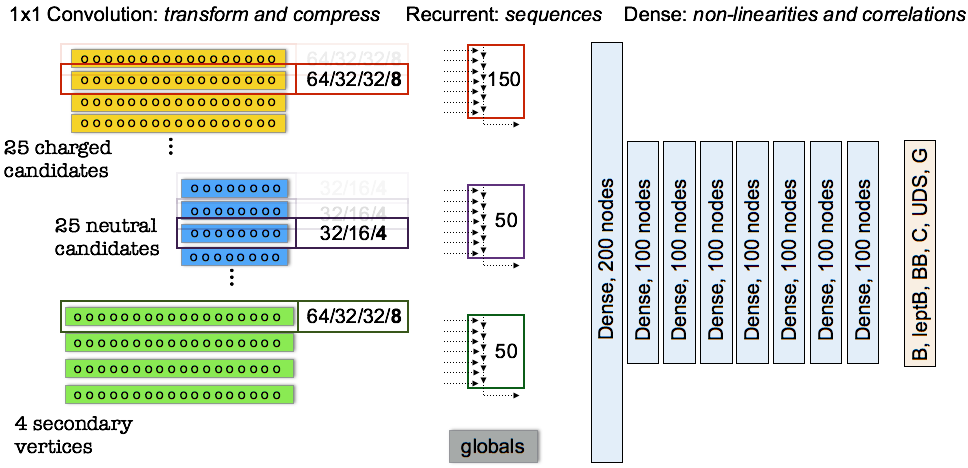
\includegraphics[width=0.8\textwidth]{chapter_5_tagging/DF.png}
\caption[Architecture of the DeepFlavour Algorithm]{\textbf{Architecture of the DeepFlavour algorithm.} Charged particle tracks, neutral particle tracks, SVs and global jet information are inserted separately in the network and compressed through $1x1$ convolutional layers. The subsequent use of recurrent sequences leads to a more flexible structure in respect of the number of objects that are present in the jet. Together with the global features, the correlations between the object can be extracted. Source: With kind permission of Jan Kieseler}
\label{fig:ch_5_DF}
\end{figure}

\subsection{Architecture}
The network structure of the DeepFlavour algorithm is shown in figure \ref{fig:ch_5_DF}. The features are divided in four groups, namely the charged candidates, the neutral candidates, the secondary vertices and the globals. The first three groups consist of several objects of which each object has the same features. Therefore, each group is arranged separately as a two dimensional feature layer. The first dimension represents the different features while the second dimension represents the various objects. A maximum of 25 charged particles, 25 neutral particles and 4 secondary vertices is given, but there is no issue for jets with less objects. The two dimensional layer is inserted into a $1x1$ convolutional layer. This kind of layer is only fully connected in the first dimension and uses shared weights in the second dimension. The $1x1$ refers to the so called filter kernel size and if a bigger filter kernel size is used, the layer performs a convolution of the input features with the so called filter, hence the name convolutional layer. A $1x1$ convolutional layer is shown in figure \ref{fig:ch_5_Conv}.\\

\begin{figure}
\centering
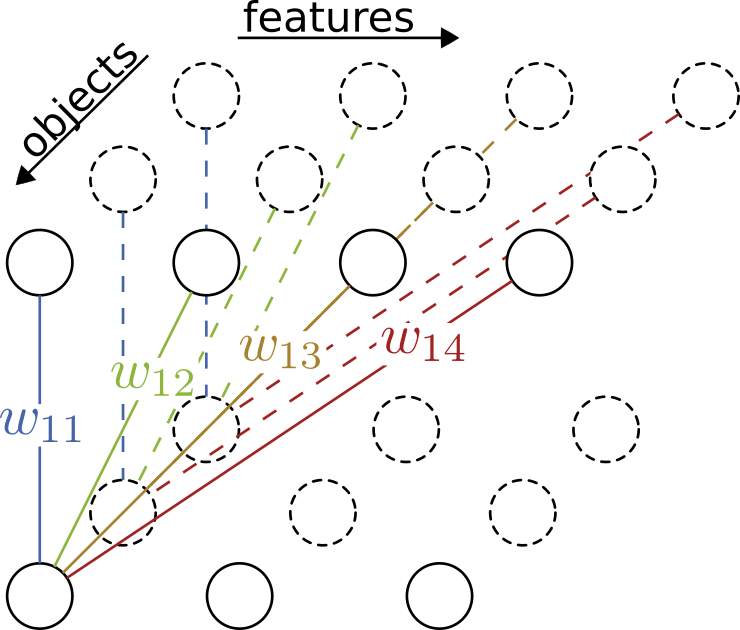
\includegraphics[width=5cm]{chapter_5_tagging/convolutional.png}
\caption[$1x1$ Convolutional Layer and LSTM Unit]{\textbf{$1x1$ convolutional layer.} Shown are three objects with four features each. The objects share their weights among themselves, the lines in the same color represent the same weights. For each filter, one output neuron is generated for each object. In this case, three filters were used.}
\label{fig:ch_5_Conv}
\end{figure}

The $1x1$ convolutional layer generates output features which are again two-dimensional. In the first dimension, new latent features are constructed while the second dimension represents the same objects as before. For the charged particles and SVs, four $1x1$ convolutional layers are connected in a row, they use 64, 32, 32 and 8 filters respectively. The neutral particles are processed in three $1x1$ convolutional layers with 32, 16 and 4 filters each. Each two-dimensional output of the last $1x1$ convolutional layer is then inserted into a long short-term memory (LSTM) \cite{LSTM} layer. The LSTM layer takes sequences of features as input, in this case the sequences are the various objects.\\

\begin{figure}
\centering
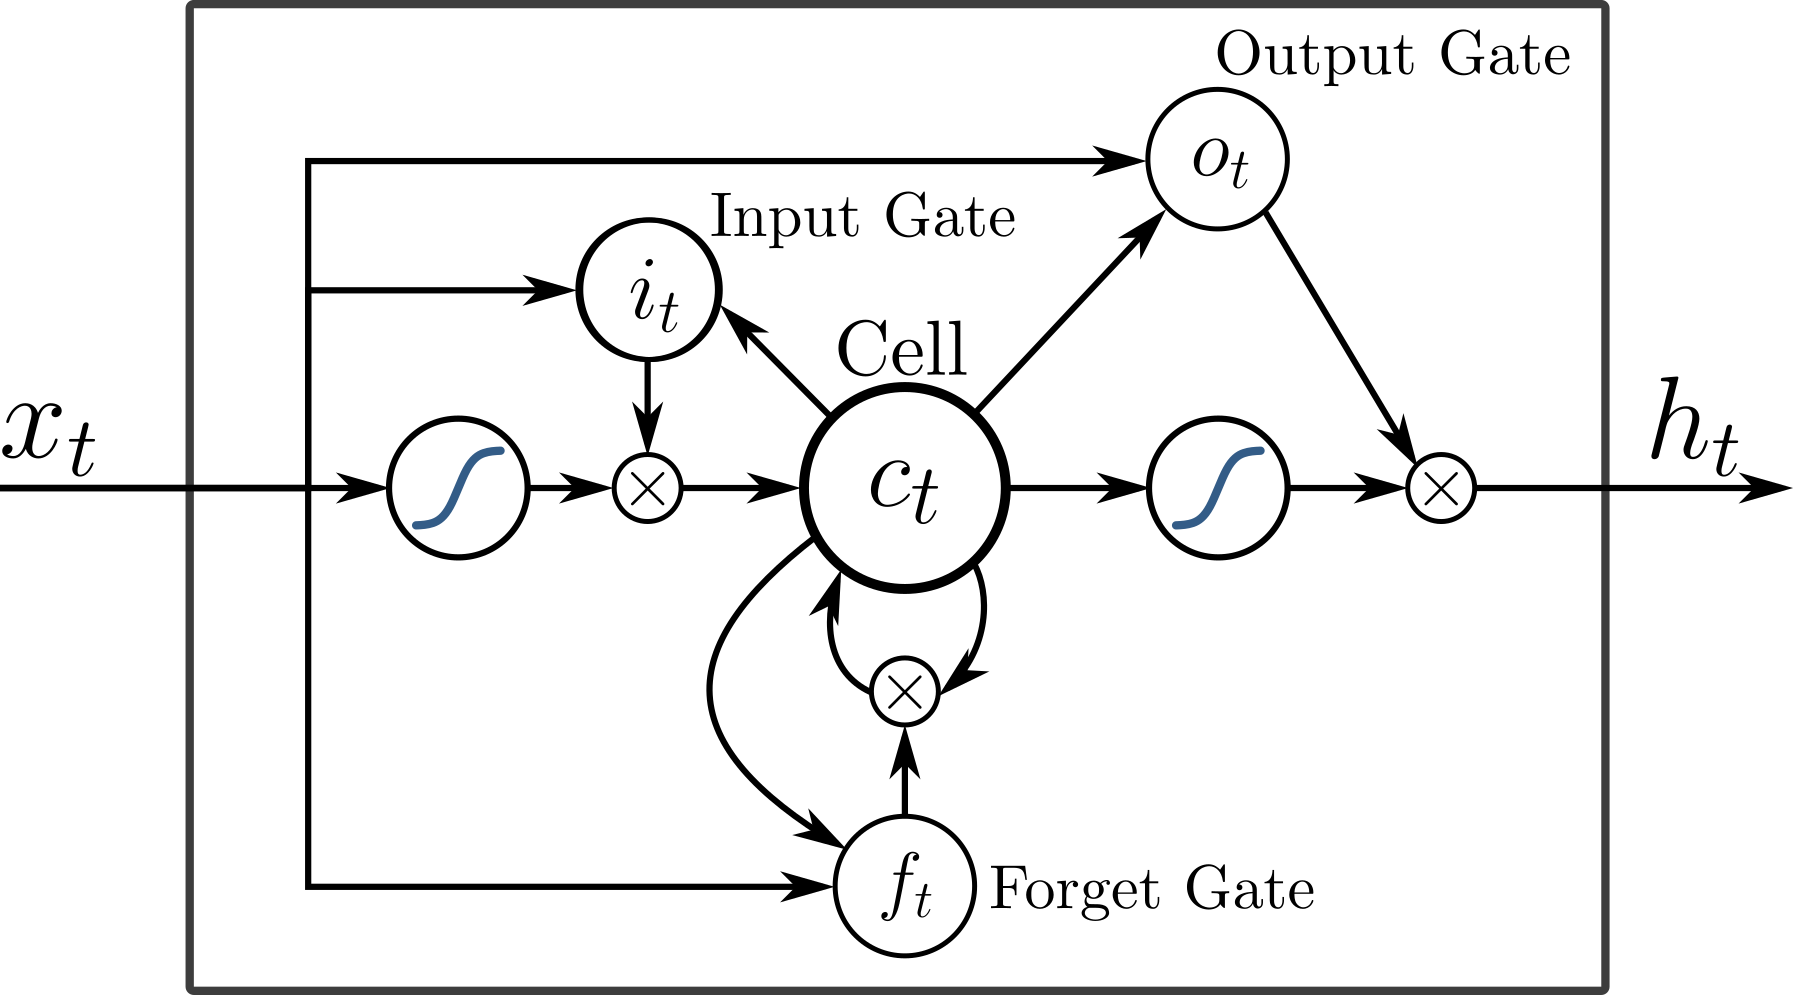
\includegraphics[width=7cm]{chapter_5_tagging/lstm.png}
\caption[Long Short-Term Memory Unit]{\textbf{Long short-term memory (LSTM) unit.} The LSTM unit transports the input vector $x_t$ to three gates. The input gate $i_t$ determines how much a new value influences the memory cell $c_t$, the forget gate $f_t$ describes the degree the value of $c_t$ is forgotten and the output gate defines the impact of $c_t$ in the output. Adapted from \cite{LSTMunit}.}
\label{fig:ch_5_LSTM}
\end{figure}

Each unit of the LSTM layer has a memory and is therefore capable of taking past sequences into account. One LSTM unit is shown in figure \ref{fig:ch_5_LSTM}. The most information can be extracted from the last sequence, therefore the sequences have to be ordered in a way that the most important sequence is inserted as the last sequence. The output of the LSTM layer is one dimensional and can be chosen freely. For the DeepFlavour algorithm, 150 units were taken for the charged particles and 50 each for the neutral particles and SVs. The outputs of the three LSTM layers from the three categories respectively are concatenated together with the features of the globals into one flat layer. These are connected to a fully connected layer with 200 neurons and followed by seven fully connected layers of 100 neurons each.\\

The LSTM layer uses hyperbolic tangent activation functions. For the other hidden layers, ReLu activation functions were used. The output layer has again sigmoid activation function. The loss function is again the categorical cross-entropy and dropout layers are applied after each hidden layer with a dropout rate of 0.1. Additionally, a batch normalization layer is applied after each hidden layer (see section \ref{sec:ch_4_perceptron} and \ref{sec:ch_4_mlp}). 


\subsection{Categories}
The categories are similar to the ones used in the DeepCSV algorithm with the difference that the DeepFlavour algorithm distinguishes between the light quarks u,d and s and gluons g, where the physics definition is used as explained in \cite{MCTruth}. Moreover it differentiates between B hadron jets where the B hadron decays leptonically or hadronically. The labeling is done in the same way as in the DeepCSV algorithm.

\subsection{Input Features}
Compared to the DeepCSV algorithm, the set of input features has been increased. 15 global features, 16 features for each charged particle, 6 features for each neutral particle and 12 features for each SV were used. For the sequential processing of the LSTM layers, the objects have to be ordered. Charged particles and SVs are sorted in respect of the 2D IP significance in descending order. Charged candidates that were used in the PV fit do not have a 2D IP significance, they are sorted in ascending order of the $\Delta R_m(cPF,SV)$ value ($\Delta R$ of the charged candidate and its closest SV in the jet). For jets without SV, the particle \pt is used in descending order as a third criterion. Neutral PF candidates are sorted as a first criterion in ascending order by their $\Delta R_m(nPF,SV)$ value and as a second criteria descending by their {\pt}.

\section{Performance of b Tagging Algorithms}
To measure the performance of a tagging algorithm, the so called receiver operating characteristic (ROC) curve can be used. The ROC curve is computed by varying the test statistic (section \ref{sec:ch_4_classification}) of the classifier output from its minimal to its maximal value. At each point the efficiency and the FPR are calculated. The ROC curve is commonly computed on simulated samples with the available labels. The performances of the DeepCSV and DeepFlavour algorithms are compared to the CSVv2 algorithm which is a well established b tagging algorithm in the CMS experiment. Their ROC curves are shown in figure \ref{fig:ch_5_Performance}. The classifier is applied at a fixed value of the test statistic, the so called working point. The working point is defined by the FPR. The loose working point (L) has a FPR of 1 \%, the medium working point (M) has a FPR of 0.1 \% and the tight working point (T) has a FPR of 0.01 \%. \\

\begin{figure}
\centering
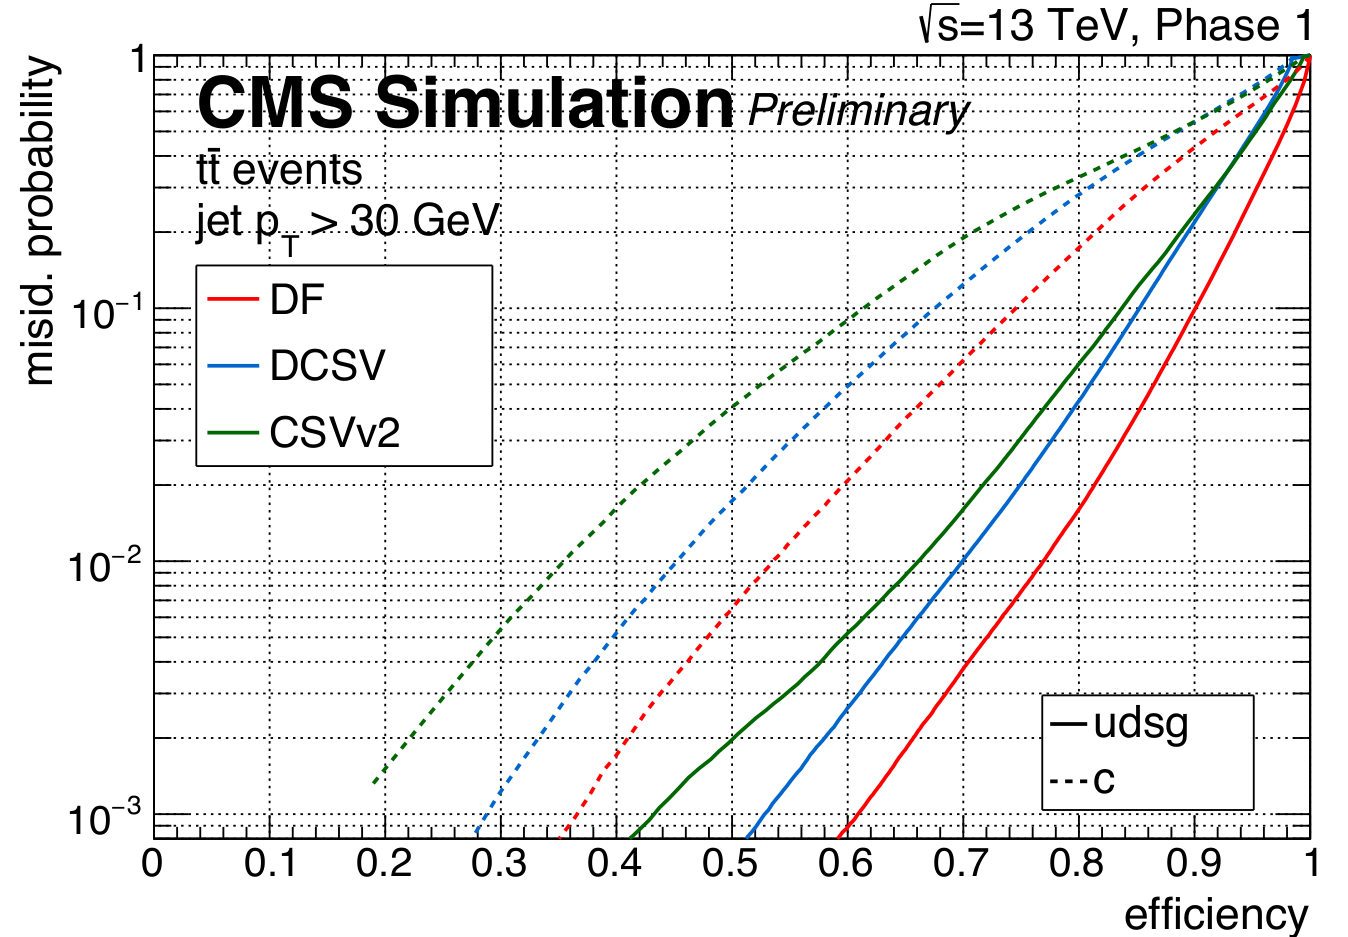
\includegraphics[width=10cm]{chapter_5_tagging/performance.png}
\caption[Architecture of the DeepFlavour Algorithm]{\textbf{Performance of b tagging algorithms.} The plot shows the misidentification probability (which is the FPR) against the b tagging efficiency measured on simulated samples. The b tagging efficiencies against light quarks and gluons (continuous lines) and c quarks (dashed lines) are shown for three different tagging algorithms. The CSVv2 algorithm has the worst performance. The DeepCSV (DCSV) is the currently proposed b tagging algorithm for CMS analyses. The DeepFlavour (DF) has the best performance, it is under development and the performance on real data is currently not known. Source: \cite{DeepFlavour}}
\label{fig:ch_5_Performance}
\end{figure}
%TODO figure not in reference! 

To calculate the efficiency in data, more complex methods have to be applied. Since these methods have model assumptions and the number of jets from data events is much more limited, they have high systematic and statistical uncertainties. With the efficiency on data $\epsilon_\textrm{data}$ and on simulated jets $\epsilon_\textrm{MC}$ on identical FPRs, a scalefactor can be computed as
\begin{equation}
SF_b = \frac{\epsilon_\textrm{data}}{\epsilon_\textrm{MC}} \quad .
\end{equation}
Scalefactors for the DeepCSV and CSVv2 algorithm computed with various methods are shown in figure \ref{fig:ch_5_Scalefactor}. As expected, the scalefactor is in the most cases lower than one, this origins from the fact that the algorithms are trained on simulation and have therefore worse performance on data. More important than a scalefactor that is close to one is a scalefactor with low uncertainty. However, scalefactors which are far from one tend to have higher uncertainties. For the DeepFlavour algorithm, there exists no official measurement of the scalefactors, but scalefactors with higher uncertainties are expected since the unselected tracks and vertices, used by the DeepFlavour algorithm are less good modeled compared to the ones used by the DeepCSV algorithm.

\begin{figure}
\centering
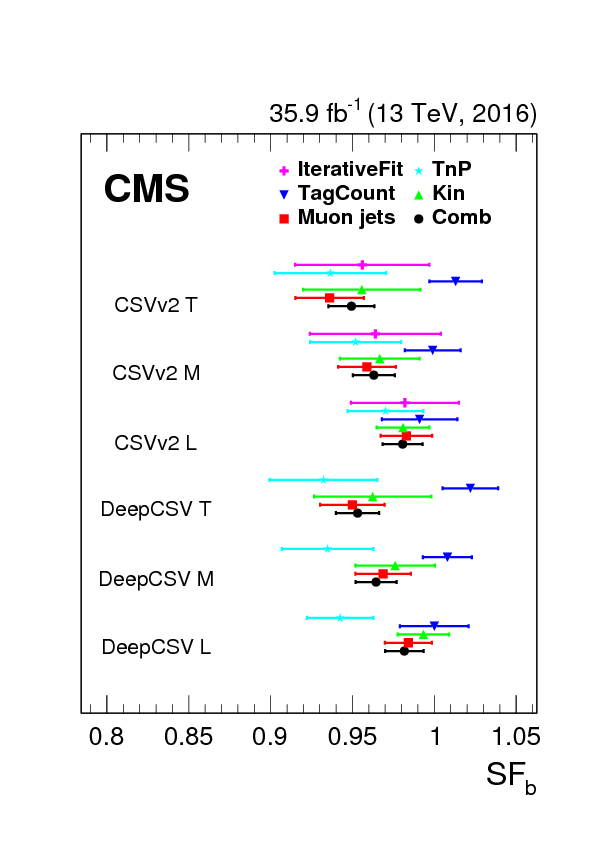
\includegraphics[width=6cm]{chapter_5_tagging/SF.png}
\caption[Scalefactors for b Tagging Algorithms]{\textbf{Scalefactor for b tagging algorithms.} The scalefactor for the b tagging algorithms at different working points are shown for five methods. The measured scalefactors agree in their uncertainties. The black dot refers to the combined value and is mainly dominated by the Muon Jets method. Source: \cite{HeavyFlavorIdentification}}
\label{fig:ch_5_Scalefactor}
\end{figure}